{\color{gray}\hrule}
\begin{center}
\section{Expérimentations}
\textbf{Dans cette section, nous verrons les expérimentations éffectuées et discuterons de leurs résulats.}
\bigskip
\end{center}
{\color{gray}\hrule}
\begin{multicols}{2}

Pour évaluer la justesse et l’efficacité de l’implémentation, il a fallu entraîner 
des architectures, ajuster leurs hyperparamètres, puis comparer les résultats obtenus avec 
ceux de Keras sur les mêmes architectures. \\

Le jeu de données MNIST a été choisi pour le premier test. Composé de 
60 000 images de chiffres manuscrits (de 0 à 9), il est l’un des jeux de données 
les plus connus pour les tâches de classification d’images. Chaque image mesure 
28x28 pixels et est en niveaux de gris. Ce jeu de données est particulièrement
populaire car il est simple à traiter et offre une grande qualité et quantité 
d’exemples, ce qui en fait une référence pour les premières expérimentations en 
apprentissage profond. \\

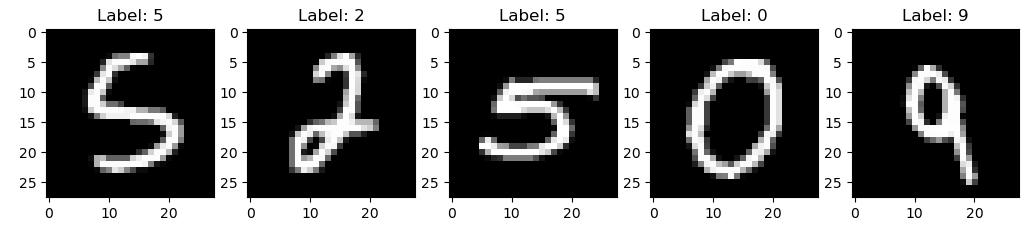
\includegraphics[width=\columnwidth]{images/mnist_samples.png}
\captionof{figure}{Exemples d'images provenant du jeu de données MNIST}
\hfill\break

Cependant, afin d’augmenter la complexité des expérimentations, le jeu de données CIFAR-10 a également 
été utilisé. Il contient 60 000 images réparties en 10 classes (avions, voitures, oiseaux, chats, cerfs, 
chiens, grenouilles, chevaux, bateaux et camions). Les images sont des photographies sous échantillonnées, qui mesurent 32x32 pixels et qui sont en couleur 
(format RGB), ce qui les rend plus complexes à traiter que celles de MNIST. La diversité des classes et le manque de corrélation 
entre elles ajoutent également de la complexité à ce jeu de données. En ce qui concerne la qualité de ces dernières,
elle est comparable à celle de MNIST. \\

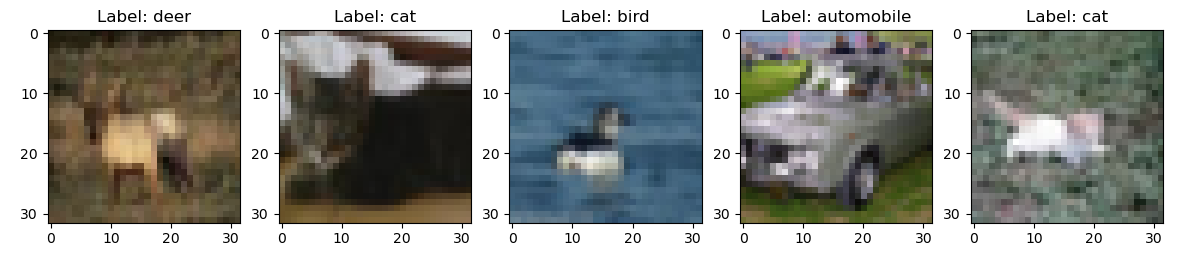
\includegraphics[width=\columnwidth]{images/cifar10_samples.png}
\captionof{figure}{Exemples d'images provenant du jeu de données CIFAR-10}
\hfill\break

\subsection{Méthode}

Le protocole expérimental est le suivant :  \\


\textbf{Pré-traitement des données} Les données sont pré-traitées 
pour être compatibles avec les modèles.\\

\textbf{Création et évaluation d’architectures avec Melpy} Des architectures sont créées 
et entraînées avec différents hyperparamètres pour identifier celle qui offre 
la meilleure généralisation.\\

\textbf{Création et entraînement des architectures avec Keras} L'architecture
sélectionnée est ensuite entraînée avec Keras de manière similaire. \\


\textbf{Comparaison des métriques finales} On compare les métriques finales d'une bibliothèque
avec celles de l'autres. \\

L’entraînement a été effectué sur un processeur Intel i5-12600K avec 32 Go de RAM. Il est important de 
noter que les temps de calcul ont pu être influencés par des processus externes indésirables. Concernant 
la métrique utilisée, seul le coût de l’architecture au fil des époques a été présenté, car il reflète 
parfaitement les performances d’un modèle. \\


\subsection{Résultats et discussion}

\subsubsection{Pré-traitement des données}

Afin d’éviter des problèmes tels que \textit{Dead ReLU}, l’explosion des gradients 
ou encore la disparition des gradients, il est nécessaire de mettre les images à l’échelle.\\

Pour ce faire, nous commençons par normaliser les données, en les mettant sur une 
échelle allant de 0 à 1, puis nous les standardisons.\\

Enfin, les étiquettes doivent être encodées. Pour cela, nous utilisons l’encodeur One-Hot.\\

\subsubsection{Sélection du modèle}

\textbf{MNIST} \\

L'architecture sélectionnée pour MNIST est la suivante : \\

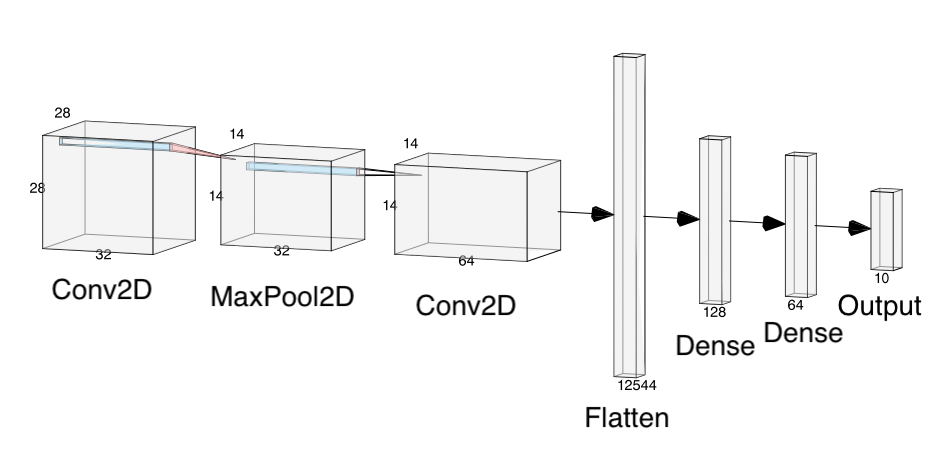
\includegraphics[width=\columnwidth]{images/mnist_nn.png}
\captionof{figure}{Réseau de neurones sélectionné pour MNIST}
\hfill\break

Comme illustré dans la Figure 10, le réseau de neurones commence par une couche de convolution qui 
génère 16 cartes de caractéristiques, suivie d’une couche de pooling qui réduit leur taille de moitié.
Ensuite, une seconde couche de convolution produit 32 cartes de caractéristiques, ensuite aplaties pour alimenter 
un MLP ayant une couche cachée composée de 128 neurones. \\

La couche cachée utilise la fonction d’activation Leaky ReLU, tandis que la sortie 
applique une fonction Softmax. Pour optimiser l'architecture, l’algorithme Adaptive Momentum (Adam) a été utilisé pour minimiser 
la fonction de coût d’entropie croisée catégorielle (Categorical Cross-Entropy). \\

Le choix a été fait sur les 5 entrainements suivants : \\

\scalebox{0.55}{
\begin{tabular}{l|c c c c c c c|}
    \cline{2-8}
                                   & $\theta$                  & $\Delta$                          & $e$           &$t/e$              & Lot     & $\gamma$             & $t$              \\
    \hline
    \multicolumn{1}{|l|}{$1$}      & 15 840               & $1C_{w, b}+2D_{w,b} = 3$     & 15            & 32sec             & 256     & $1^{-4}$             &08min 01sec           \\             
    \multicolumn{1}{|l|}{$2$}      & 201 226              & $1C_{w, b}+2D_{w,b} = 3$     & 15            & 02min 23sec       & 256     & $1^{-4}$             &35min 58sec           \\ 
    \multicolumn{1}{|l|}{$3$}      & 806 394              & $2C_{w, b}+2D_{w,b} = 4$     & 15            & 01min 53sec       & 256     & $1^{-4}$             &28min 22sec           \\ 
    \multicolumn{1}{|l|}{$4$}      & 1 624 842            & $2C_{w, b}+4D_{w,b} = 6$     & 10            & 04min 42sec       & 256     & $1^{-4}$             &47min 03sec \\
    \multicolumn{1}{|l|}{$5$}      & 1 615 466            & $2C_{w, b}+2D_{w,b} = 4$     & 10            & 04min 40sec       & 256     & $1^{-4}$             &46min 49sec  \\
    \hline
\end{tabular}}
\captionof{table}{Entrainements éffectués sur MNIST avec Melpy} \\

{\scriptsize
$\theta$ étant le nombre de paramètres dans l'architecture\\

$\Delta$ étant la prodondeur de l'architecture avec $C$ une couche de convolution, D une couche entièrement connectée, $w$ l'utilisation de poids et $b$ l'utilisation de biais \\

$e$ étant le nombre d'époques passés pour entrainer l'architecture \\

$Lot$ étant le nombre d'entrées entrainées sur une passe avant et arrière \\

$\gamma$ étant le taux d'apprentissage utilisé dans l'algorithme d'optimisation \\

$t$ étant le temps qu'il a fallu pour entrainer l'architecture \\

$t/e$ étant le temps passé en moyenne sur une époque \\
} \\
\textit{La taille des lots et le taux d’apprentissage restent ici inchangés, car ils se sont révélés significativement plus stables 
que d'autres configurations testées, n'apportant pas d’informations pertinentes sur les entrainements.} \\


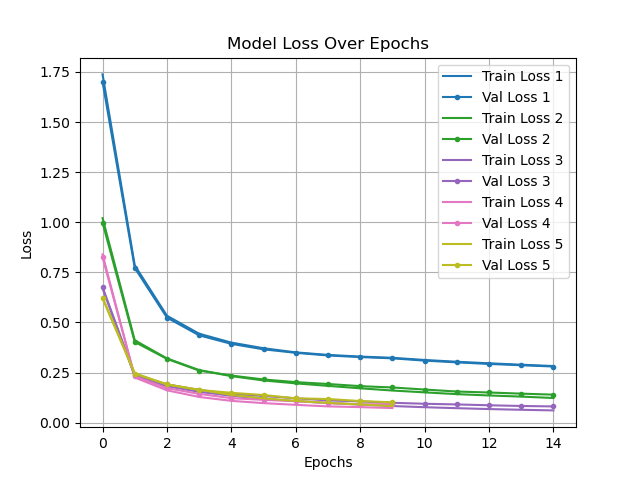
\includegraphics[width=\columnwidth]{images/mnist_losses.png}
\captionof{figure}{Le coût de l'architecture au fil des époques}
\hfill\break

Comme l’illustre la Figure 13, les modèles 3, 4 et 5 présentent des performances similaires. 
Cependant, le modèle 3 est sélectionné en raison de sa rapidité d’exécution sur une 
époque (voir Table 2). \\

En dehors de la sélection d’un modèle à comparer avec Keras, nous pouvons relever les informations suivantes concernant les différents entrainements :
\begin{itemize}
\item \textbf{Nombre de paramètres} : Le nombre de paramètres influence significativement le temps nécessaire pour réaliser une époque.
\item \textbf{Complexité du modèle} : Les modèles plus complexes tendent à mieux détecter les motifs. Cependant, cette complexité devient moins efficace 
lorsque le nombre de neurones ou la profondeur de l’architecture devient excessif.
\end{itemize} 
\hfill\break

\textbf{CIFAR-10} \\

L'architecture sélectionnée pour CIFAR-10 est la suivante : \\

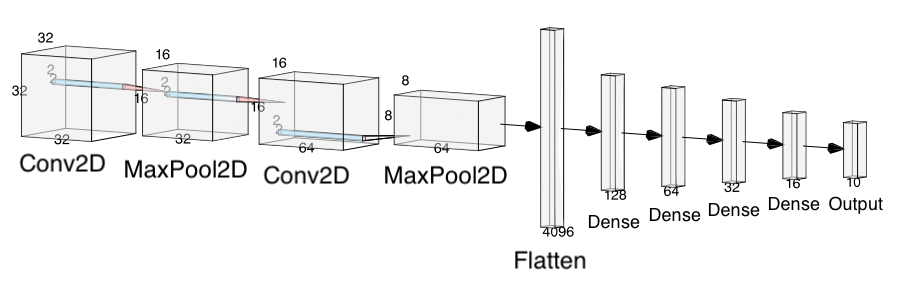
\includegraphics[width=\columnwidth]{images/cifar10_nn.png}
\captionof{figure}{Réseau de neurones sélectionné pour CIFAR-10}
\hfill\break


Comme illustré dans la Figure 14, le réseau de neurones débute par une couche de convolution générant 32 cartes de caractéristiques, suivie d’une couche de pooling réduisant leur taille de moitié. 
Cette opération est répétée une seconde fois, avec comme seule différence la couche de convolution produisant cette fois 64 cartes de caractéristiques.
Celles-ci sont ensuite aplaties pour alimenter un MLP constitué de 4 couches cachées contenant respectivement 128, 64, 32 et 16 neurones chacune. \\

Les couches cachées utilisent la fonction d’activation Leaky ReLU, tandis que la sortie 
applique une fonction Softmax. Pour optimiser l'architecture, l’algorithme Adam a été utilisé pour minimiser 
la fonction de coût d’entropie croisée catégorielle. \\

Le choix a été fait sur les 6 entrainements suivants : \\

\scalebox{0.515}{
\begin{tabular}{l|c c c c c c c|}
    \cline{2-8}
                                   & $\theta$                  & $\Delta$                     & $e$           &$t/e$        & Lot     & $\gamma$             & $t$              \\
    \hline
    \multicolumn{1}{|l|}{$1$}      & 1 056 376            & $4C_{w}+2D_{w,b} = 6$        & 20            & 09min 50sec & 128     & $5^{-5}$             &03h 16min 59sec           \\
    \multicolumn{1}{|l|}{$2$}      & 2 107 146            & $2C_{w}+2D_{w,b} = 4$        & 20            & 17min 24sec & 128     & $1^{-5}$             &05h 48min 14sec           \\
    \multicolumn{1}{|l|}{$3$}      & 2 107 146            & $2C_{w}+2D_{w,b} = 4$        & 35            & 15min 38sec & 128     & $5^{-5}$             &09h 07min 21sec           \\
    \multicolumn{1}{|l|}{$4$}      & 2 107 146            & $2C_{w}+2D_{w,b} = 4$        & 50            & 08min 12sec & 256     & $5^{-5}$             &06h 50min 36sec          \\
    \multicolumn{1}{|l|}{$5$}      & 2 117 866            & $2C_{w}+2D_{w,b} = 4$        & 100           & 10min 27sec & 128     & $5^{-5}$             &17h 26min 00sec           \\
    \multicolumn{1}{|l|}{$6$}      & 8 398 698            & $2C_{w,b}+2D_{w,b} = 4$      & 50            & 08min 34sec & 64      & $5^{-6}$             &07h 08min 29sec           \\
    \multicolumn{1}{|l|}{$7$}      & 544 122              & $2C_{w,b}+5D_{w,b} = 7$      & 50            & 05min 53sec & 64      & $5^{-5}$             &04h 54min 52sec           \\
    \multicolumn{1}{|l|}{$8$}      & 8 408 442            & $2C_{w,b}+5D_{w,b} = 7$      & 50            & 10min 26sec & 64      & $5^{-5}$             &08h 42min 17sec           \\
    \hline
\end{tabular}}
\captionof{table}{Entrainements éffectués sur CIFAR-10 avec Melpy} \\

{\scriptsize
$\theta$ étant le nombre de paramètres dans l'architecture\\

$\Delta$ étant la prodondeur de l'architecture avec $C$ une couche de convolution, D une couche entièrement connectée, $w$ l'utilisation de poids et $b$ l'utilisation de biais \\

$e$ étant le nombre d'époques passés pour entrainer l'architecture \\

$Lot$ étant le nombre d'entrées entrainées sur une passe avant et arrière \\

$\gamma$ étant le taux d'apprentissage utilisé dans l'algorithme d'optimisation \\

$t$ étant le temps qu'il a fallu pour entrainer l'architecture \\

$t/e$ étant le temps passé en moyenne sur une époque \\
} \\

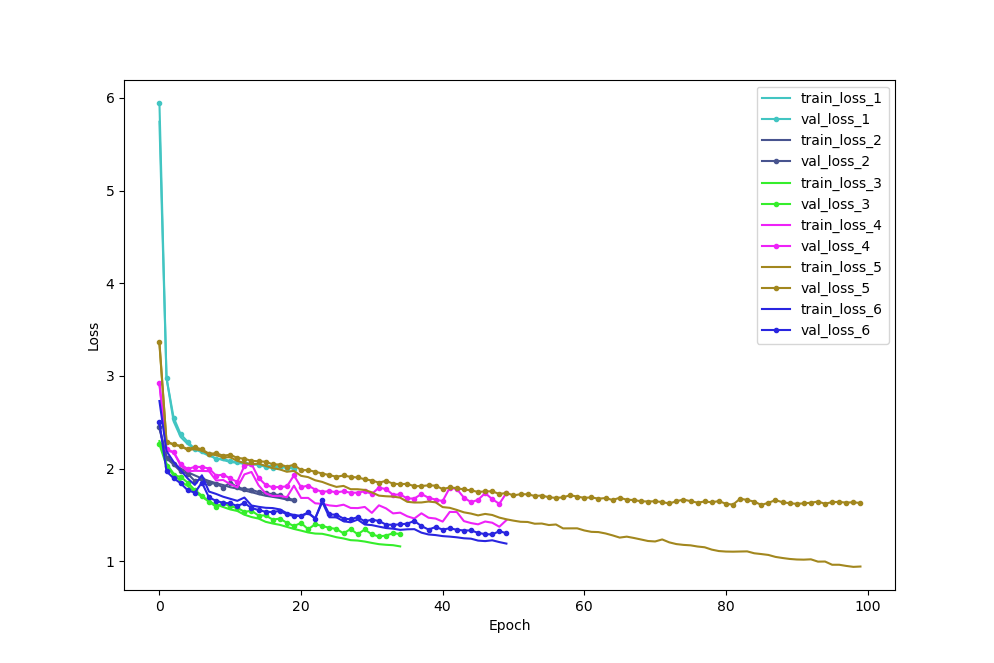
\includegraphics[width=\columnwidth]{images/cifar_10_losses.png}
\captionof{figure}{Le coût de l'architecture au fil des époques}
\hfill\break

Comme le montre la Figure 15, les modèles 3, 7 et 8 se démarquent comme 
les plus performants. Parmi eux, c'est bien le modèle 7 qui a été retenu. Ce choix repose sur un 
compromis entre la qualité de sa généralisation, son temps d’entraînement réduit et 
son efficacité dès le début de ce dernier. \\

À l'instar des entrainements sur MNIST, nous pouvons relever les informations suivantes à partir de l'ensemble des entrainements sélectionnés pour CIFAR-10 :  
\begin{itemize}
    \item \textbf{Taille des lots} : Elle influence de manière significative le temps de calcul par époque ainsi que le nombre d’itérations nécessaires pour atteindre 
    la convergence.
    \item \textbf{Capacité de généralisation} : La taille des lots influence également la capacité du modèle à bien généraliser sur des données non vues, à condition que le modèle ne soit pas trop complexe.
    \item \textbf{Couches de pooling} : L’intégration de couches de pooling à des positions intéressantes dans l’architecture peut compenser le temps de calcul, 
    bien que cela se fasse au détriment de la quantité d’informations utilisé pour l’apprentissage.
\end{itemize}
\hfill\break


\subsubsection{Comparaison des résultats}

Afin d’évaluer les performances de Melpy dans l’utilisation des CNNs, nous comparons cette bibliothèque avec Keras, une autre bibliothèque de deep learning, reconnue pour la simplicité de son utilisation. \\

Pour ce faire, ce sont les architectures sélectionnées plus tôt qui serviront de référence.\\

Observons les différences entre les métriques calculées durant l’entraînement pour chaque jeu de données : \\

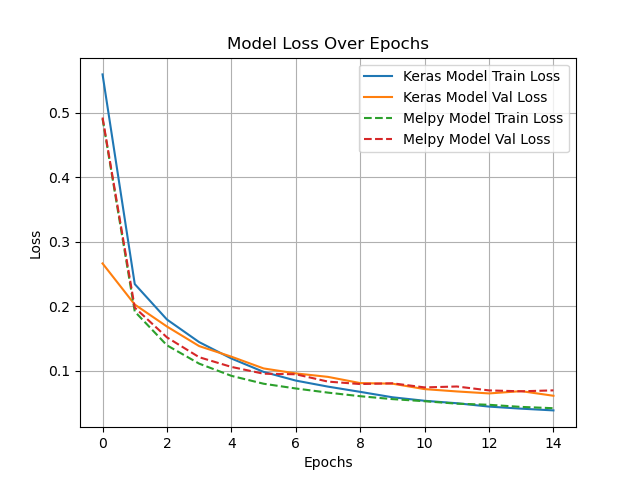
\includegraphics[width=\columnwidth]{images/mnist_loss_comparison.png}
\captionof{figure}{Comparaison du coût entre Melpy et Keras sur MNIST}
\hfill\break

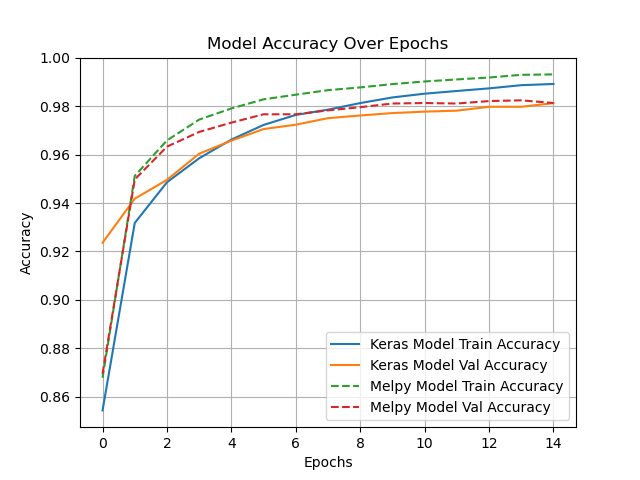
\includegraphics[width=\columnwidth]{images/mnist_accuracy_comparison.png}
\captionof{figure}{Comparaison de la précision entre Melpy et Keras sur MNIST}
\hfill\break

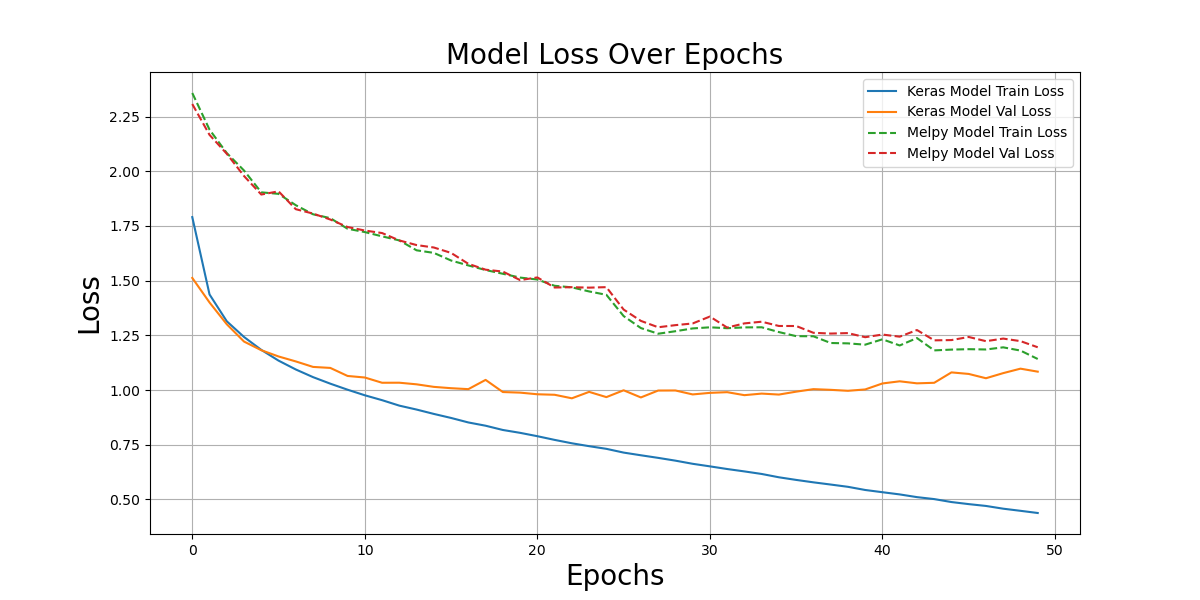
\includegraphics[width=\columnwidth]{images/cifar10_loss_comparison.png}
\captionof{figure}{Comparaison du coût entre Melpy et Keras sur CIFAR-10}
\hfill\break

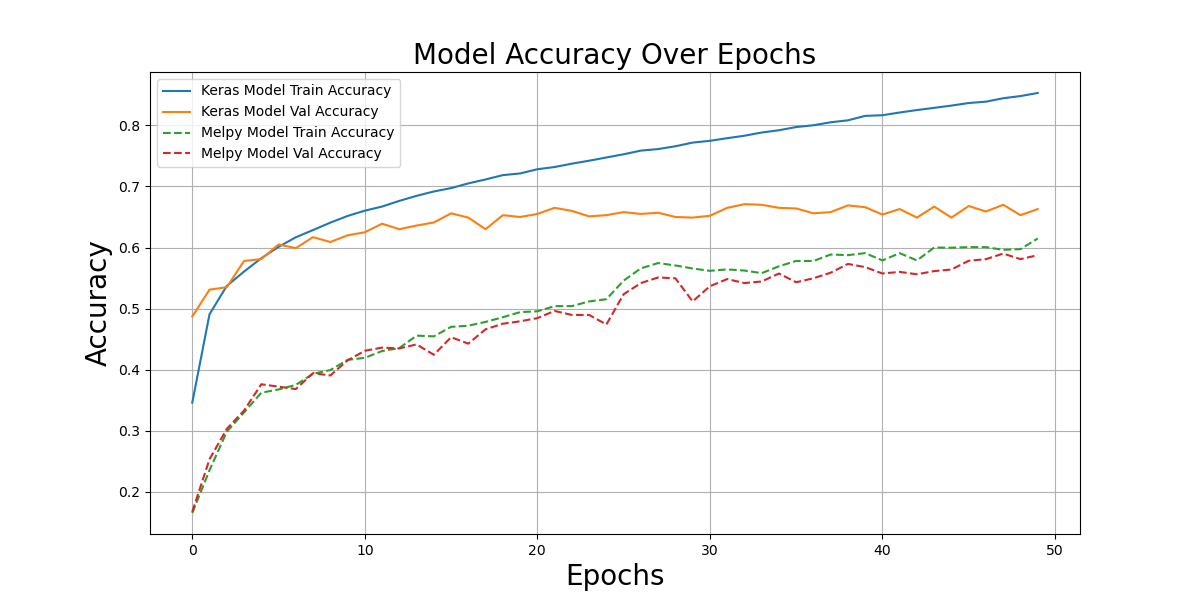
\includegraphics[width=\columnwidth]{images/cifar10_accuracy_comparison.png}
\captionof{figure}{Comparaison de la précision entre Melpy et Keras sur CIFAR-10}
\hfill\break

Comme le montrent les Figures 16 à 19, les résultats varient considérablement d’un jeu de données à 
un autre. Cette variation peut être attribuée à une légère divergence dans le calcul du gradient au 
niveau des couches de convolution. En effet, des tests comparant les résultats des opérations mathématiques 
implémentées dans Melpy à celles de TensorFlow (la bibliothèque utilisée par Keras pour ses calculs) ont 
révélé une différence moyenne allant de 0,4 à 0,6 entre les gradients pour chaque valeur d’entrée. Bien que 
faible à l’échelle individuelle, cette divergence devient significative en raison du grand nombre de valeurs 
impliquées. Par exemple, pour un gradient de taille (1, 3, 32, 32), la somme des erreurs peut atteindre 1800, 
alors que les autres opérations testées présentent des écarts proches de zéro.

Cette différence s’explique notamment par la méthode de différentiation automatique\cite{autodiff} utilisée par TensorFlow, 
qui génère des gradients avec une grande précision, et par des méthodes de normalisation intégrées. Ces dernières 
redistribuent plus équitablement les gradients accumulés lorsque les fenêtres de convolution se chevauchent, 
évitant ainsi des calculs biaisés. Toutefois, malgré ces limitations, le calcul actuel de la propagation 
arrière dans Melpy reste suffisant pour obtenir des résultats corrects.

En effet, sur le jeu de données MNIST, l’architecture entraînée avec Keras a obtenu des performances équivalentes 
à celles de Melpy, atteignant une précision proche de 98\% sur le jeu de données de validation. En revanche, sur 
le jeu de données CIFAR-10, bien que l’apprentissage ait été significativement plus lent avec Melpy, l’architecture 
entraînée avec cette dernière a su converger vers une précision d’environ 65\% sur le jeu de données de validation, 
résultat comparable à celui obtenue avec Keras. \\

On peut également relevé le temps d'execution qu'il a fallu à Keras sur les mêmes configurations que Melpy : \\

\scalebox{0.95}{
\begin{tabular}{l|c c|}
    \cline{2-3}
                                     & Melpy                  & Keras                                \\
    \hline
    \multicolumn{1}{|l|}{MNIST}      & 28min 22sec            & 01min 15sec                    \\
    \multicolumn{1}{|l|}{CIFAR-10}   & 04h 54min 52sec        & 10min 43sec                    \\

    \hline
\end{tabular}}
\captionof{table}{Durées des entrainements éffectués sur CIFAR-10 et MNIST} \\

La différence importante dans les temps d’exécution (voir Table 4) s’explique par les optimisations intégrées à Keras. 
La bibliothèque compile les modèles en code machine via TensorFlow, ce qui accélère l’exécution 
des opérations. De plus, Keras exploite plus efficacement le parallélisme, 
ce qui améliore de surcroit les performances des calculs.

En revanche, Melpy, dans son état actuel, n’intègre pas encore de telles optimisations. 
Ses opérations restent dépendantes de l’interprétation directe de Python, ce qui allonge 
les temps d’exécution. \\

\end{multicols}